\documentclass[a4paper,11pt]{article}
\usepackage{macros-ohp}
\usepackage{blindtext}
\usepackage{graphicx}
\usepackage{subcaption}
\usepackage{float}

%Please make sure the tex is compiled twice to have all the background images displayed correctly.

\title{\Huge \textbf{The TIV model: robustness with respect to parameter variation}}

\author{\Huge Amir Farid Kaveh\\
	\Large Supervised by Prof James McCaw \& Dr Pengxing Cao \\
	\Large The University of Melbourne\\
}
\date{28/02/2019}

\linespread{1.5}

\begin{document}
	\begin{titlingpage}
	\tikz[remember picture,overlay] \node[opacity=1,inner sep=0pt] at (current page.center){
\includegraphics[width=\paperwidth,height=\paperheight]{imgs/background.png}};
	\vspace*{3.5cm}
	{\let\newpage\relax\maketitle}
	\vspace*{\fill}
	\begin{textblock*}{140mm}(40mm,200mm)
			\begin{center}
				\begin{small}
		Vacation Research Scholarships are funded jointly by the Department of Education and Training
and the Australian Mathematical Sciences Institute.
				\end{small}
			\end{center}
	\end{textblock*}

	\end{titlingpage}


\section*{Abstract}
Multidrug therapy is the practice of treating an infection with more that one class of drug. A 2018 paper by Melville et al. aims to simulate the effect of this type of therapy on influenza A infection using a variant of the Target-cell-limited (TIV) model. Here we aim to test the robustness of the TIV model by using a different variation to simulate the same scenarios as their paper and then comparing our results with theirs. 
\section*{Introduction}
Viruses are microscopic entities composed of one type of nucleic acid, RNA or DNA, encased in a coat of protective proteins called the capsid. Viruses can be pathogenic. They are unable to generate energy or replicate independently and are completely inert outside a host cell. Once inside a host cell, a virus will hijack the cell's biochemical machinery in order to express their genome and replicate.$^{[27]}$ 

Multi-drug therapy (MDT) is the practice of treating an infection with more than one class of drug. It is currently in use against diseases such as HIV$^{[1]}$ and leprosy$^{[2]}$ . MDT provides two main benefits. First, it provides an additional barrier to the development of drug resistance in pathogens$^{[8]}$, and second, drugs used in combination can be synergistic, i.e. they may be more effective when used in tandem than when acting alone. They could also be antagonistic. It is the latter of these two potential benefits that concerns this paper. 

There are currently three classes of antiviral drugs approved by the FDA for use in Influenza therapy. One of these classes, amantadine, is no longer recommended by the CDC. This is due to the development of resistance in 100\% of seasonal H3N2 and pandemic flu samples tested in 2009.$^{[3]}$ This is an unsurprising development since the Influenza virus has high mutation rates $^{[4][5]}$ and is able to quickly develop resistance to antivirals.$^{[6][7]}$ 

The threat posed by drug resistant viruses, along with the possibility of synergistic behaviour motivates the study of MDT as a potential method of treating influenza. This avenue has been the subject of some exploration before$^{[6][8]}$; of particular interest to us is the Melville et al, 2018 paper focusing on the action of pairs of antiviral drugs on the progression of Influenza infection in vitro as predicted by a variant of the Target cell limited model. The Target cell limited model is a system of ordinary differential equations (ODEs) that describes the essential interactions between the healthy target cells (denoted by T), infected cells (denoted by I), and viral load (denoted by V) within a host. These equations are often referred to as the TIV model.  

The variant of the \textit{TIV} model used can be generalized as follows, 

\begin{align*}
\dot{T} &= -\beta TV \\
\dot{E}_1 &= \beta TV - \frac{n_E}{\tau_E}E_1 \\
\dot{E}_i &= \frac{n_E}{\tau_E}(E_{i-1}-E_i) \\ 
\dot{I}_1 &= \frac{n_E}{\tau_E}E_{n_E}-\frac{n_I}{\tau_I}I_1\\
\dot{I}_i &= \frac{n_I}{\tau_I}(I_{i-1}-I_{i}) \\
\dot{V} &= p\sum_{i=1}^{n_I}I_i - cV,
\end{align*}

 The parameters, in order of their appearance, are $\beta$, the infectivity, or the rate at which the virions infect healthy cells, $n_E$ the number of eclipse phase compartments, $\tau_E$ the mean life time of the eclipse phase, $n_I$ the number of infectious phase compartments, $\tau_I$ is the mean life time of a cell after it enters the infectious phase, $p$ is the rate at which infectious cells produce virions and $1/c$ is the mean life time of virions. 

The Melville et al. study used this model with $n_E =30$, and $n_I = 100$. We will refer to this as the original model. In our study we will be reducing the number of compartments to ten and one respectively. We also reduce the lifetime of infected cells by a factor of five. This will be the altered model from here on. All other parameters are unchanged from the Melville et. al. study; with the possible exception of the initial conditions for the infected cell compartments, eclipse phase compartments and viral load. We set $I_i(0)=E_i(0)=0$. All other parameters can be found in the table below. 


\begin{center}
\begin{tabular}{ c c c }
 $T_0$ & initial number of target cells & $10^6$ \\
 $V_0$ & initial viral load & $10^6 \hspace{1mm} \mathrm{TCID}_{50}$ \\
 $c$ & viral clearance rate & 0.13 /h \\  
 $\tau_E$ & mean eclipse phase duration & 6.6 h\\
 $\tau_I$ & mean infectious phase duration & 49/5\\
 $n_E$ & number of eclipse phase compartments & 10\\
 $n_I$ & number of infectious phase compratments & 1\\
 $p$ & viral production rate & 176 $\mathrm{TCID}_{50}(\mathrm{h \cdot cell})^{-1}$\\
 $\beta$ & infection rate & $4.260\times10^{-4} (\mathrm{h \cdot TCID_{50}})^{-1}$
\end{tabular}
\end{center}




Initially we only made the changes $n_E$ and $n_I$, but later decided to reduce $\tau_I$ in order to keep the untreated infection duration comparable between the two models. 

All the results obtained from the original model are taken from the study by Melville K., Rodriguez T., and Dobrovolny H. M. who also own the copyrights. Their paper was published in frontiers in Pharmocology on 23 October 2018 under a Creative Commons Attribution License (CC BY). 

This is a non-linear system of ODEs for which there is no known analytic solution, so we turn to numerical methods. Variants of the TIV model are widespread throughout the literature and are commonly used to model viral infections including influenza$^{[9][10][11]}$ and HIV$^{[12]}$. An important parameter that is not explicitly present in the equations is the basic reproductive ratio, $R_0 = \beta T(0)p\tauI/c$. Intuitively this is the average number of healthy cells an infected cell will infect before it dies off. If $R_0 > 1$ then there will be an infection, but where $R_0 < 1$ the initial viral load/infected cell population will fail to grow.

The aim of this study is to examine the response of the viral load curve to combination therapy with pairs of antivirals as predicted by the two variations of the TIV model we have described. There are many variations of this system of equations. Without data we cannot determine which, if any, of these renditions gives us the best model. Hence, if we hope to motivate laboratory testing based on predictions made by this system, it is crucial to demonstrate that there is at least qualitative agreement between the predictions of different variations. The ultimate goal is to address this concern. 

\begin{figure}
    \centering
    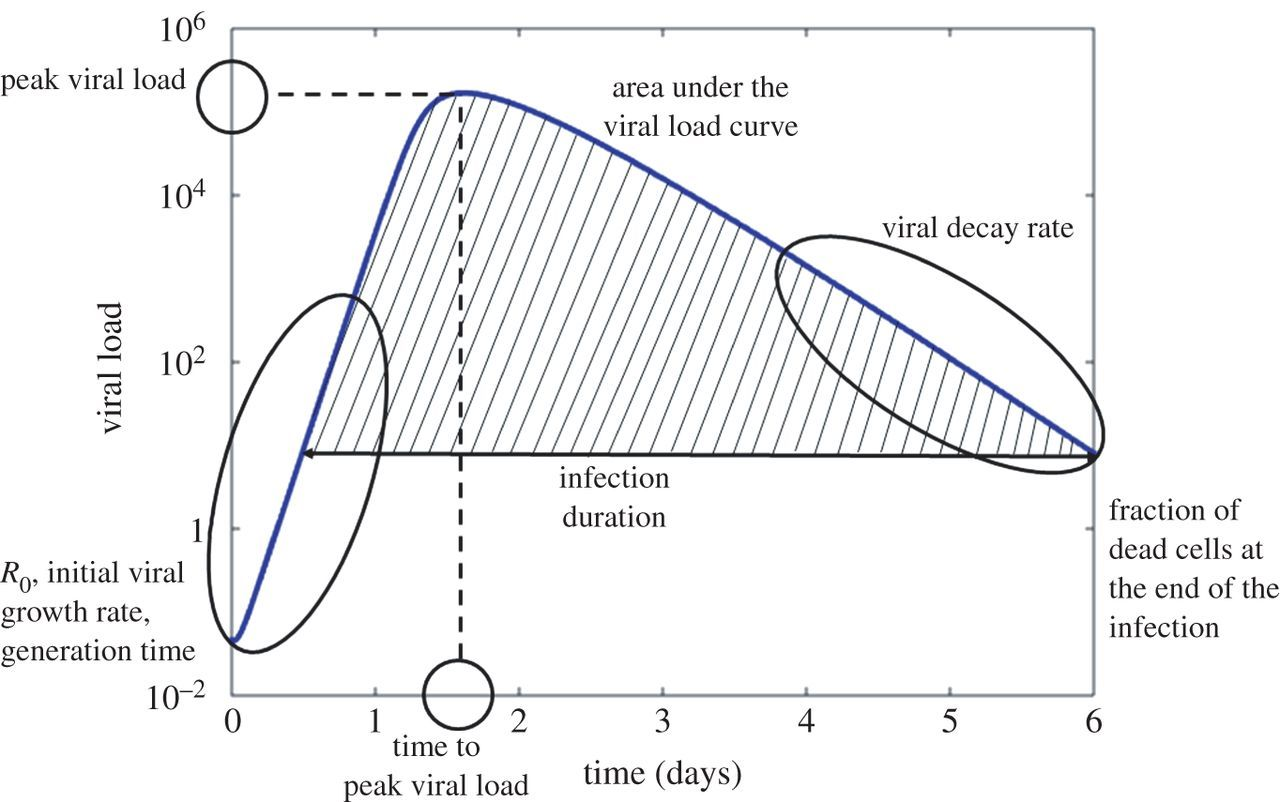
\includegraphics[scale = 1.1]{viralcurve.jpg}
    \caption{\small A typical viral load curve with $R_0 > 1$. Important attributes are highlighted. Downloaded from https://royalsociety.org on 30/01/19
}
    \label{fig:my_label}
\end{figure}

\section*{Methods}
We will be interested in examining how MDT effects the time series for $V(t)$ at a range of doses of pairs of drugs with different mechanisms of action. Figure 1 shows the typical behaviour of the viral load curve for the TIV model with $R_0 > 1$, along with it's important features. We will be examining the peak viral load, which is correlated with symptom severity, and the infection duration, which indicates the time scale of the infection.$^{[9]}$ 

As previously mentioned, there are currently only two classes of antivirals recommended by the CDC for use against influenza.$^{[13]}$ However, as new antivirals are developed$^{[14]}$, clinicians will need to adopt treatment plans that limit the emergence of drug resistance. With this in mind, we examine a broad range of drug actions as follows. 

\begin{itemize}
    \item Reducing infectivity: these are drugs that reduce $\beta$, so when modelling them we will set $\beta \rightarrow (1-\epsilon)\beta$, where $\epsilon$ is the efficacy of the drug, to be discussed shortly. These are drugs that restrict entry of virions into the cell/
    \item Protecting target cells: here we also set $\beta \rightarrow (1-\epsilon)\beta$, but only in the equation for $\dot{E}_1$. This represents an antiviral that does not work to prevent entry into the cell, but hinders intracellular processes that lead to virus replication. It is important to note that this implies the existence of another, 'hidden', compartment; since cells are removed from the target cell population but do not instantly move into the eclipse phase. This was shown to be the best method for modelling the effects of amantadine.$^{[10]}$ 
    \item Reducing virion production rate: to model drugs that have this effect we set $p \rightarrow (1-\epsilon)p$. This is considered to be the best way to model the mechanism of action for Neurominidase inhibitors.$^{[15][16]}$
    \item Decreasing the average virion life time: here we have $c \rightarrow c/(1-\epsilon)$. This can be the effect of a drug that simulates the function of the adaptive immune response$^{[17][18]}$ or one that inactivates virus.$^{[19]}$
    \item Increasing the length of the eclipse phase: for such a mechanism we set $\tau_E \rightarrow \tau_E/(1-\epsilon)$. This can be linked to several effects such as decreasing the rate of protein production or RNA.$^{[20]}$
    \item Decreasing the mean lifetime of infected cells: here we set $\tau_I \rightarrow (1-\epsilon)\tau_I$. This could for example be a drug that stimulates cytotoxic T lymphocytes.$^{[21]}$
\end{itemize}



The efficay of drugs, $\epsilon$, is related to the $E_{max}$ model:$^{[21]}$ $$\epsilon = \frac{\epsilon_{max}D^\gamma}{D^\gamma+\mathrm{IC}_{50}^\gamma},$$

where $\epsilon_{max}$ is the maximum of the drug, which we take to be one such that we have access to the widest range of behaviours for each class of antiviral. $\mathrm{IC}_{50}$ is the dose required to achieve $\epsilon = \epsilon_{max}/2$ for each drug and $D$ is the dose. $\gamma$ is the Hill coefficient. It is biologically determined by the number of binding interactions that are required for the drug to take effect. We can take this to be one for influenza antivirals.$^{[21][10]}$

Here and in the Melville et al. study, $\mathrm{IC}_{50}$ is set to one, such that doses are in terms of this measure for each drug. 


We will be looking at pairs of drugs, with efficacy $\epsilon_1$, $\epsilon_2$, at various doses, which will determine each efficacy as described. There are methods to quantify the synergy/antagony between each pair of drug actions,$^{[8]}$ however that is beyond the scope of this report. We will simply be interested in comparing the behaviour of each pair as predicted by the two models given above. 

\section*{Results}
Figure 2 shows the viral load in the untreated state, as well as when treated by a drug that reduces infectivity, one that reduces viral production rate, and both drugs in conjunction. In both models, reducing $\beta$ has little or no effect on the peak viral load, but shifts the time to peak viral load to the right. Reducing the production rate has significant effect on the peak viral load under both models, and the effect of MDT seems to be a simple overlapping of the two effects. Under the altered model, however, higher doses also lead to significantly longer infection duration, while this is not the case for the original. 

\begin{figure}[ht]
    \centering
    \begin{subfigure}{0.4\textwidth}
    
    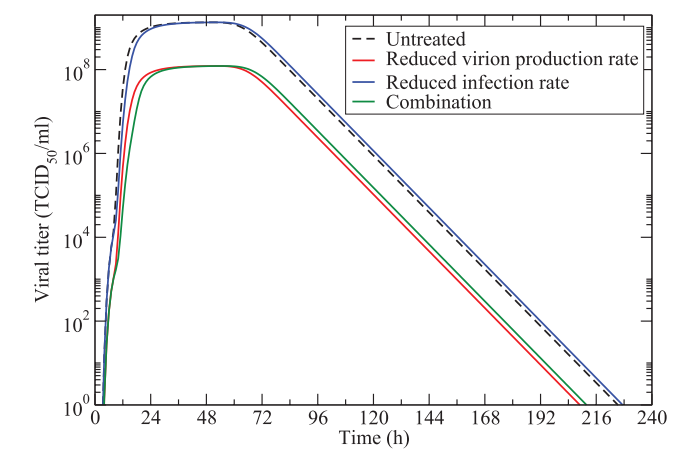
\includegraphics[width=\textwidth]{treatm10.png}
    \end{subfigure}
    \begin{subfigure}{0.35\textwidth}
    
    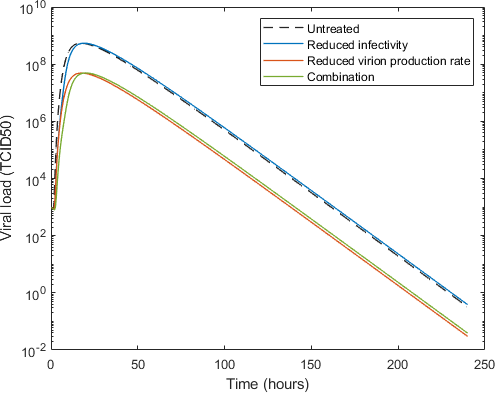
\includegraphics[width=\textwidth]{treat10.png}
    \end{subfigure}
    
    \begin{subfigure}{0.4\textwidth}
    
    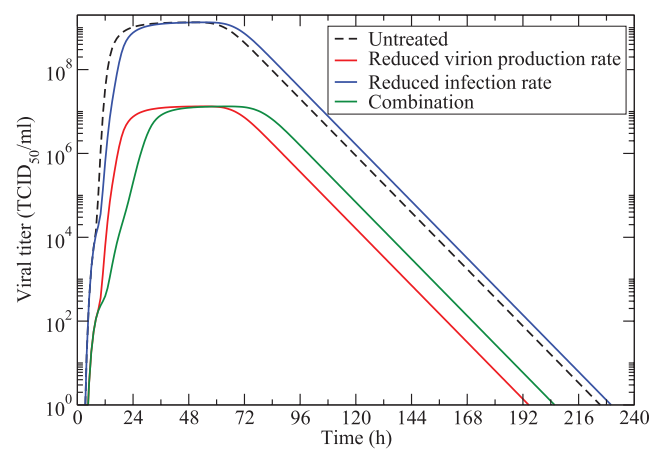
\includegraphics[width=\textwidth]{treatm100.png}
    \end{subfigure}
    \begin{subfigure}{0.35\textwidth}
    
    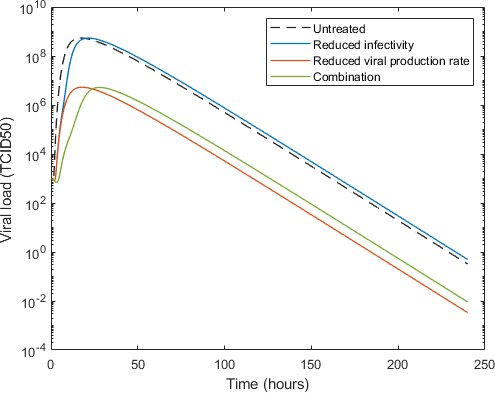
\includegraphics[width=\textwidth]{treat100.png}
    \end{subfigure}
    
    \begin{subfigure}{0.4\textwidth}
    
    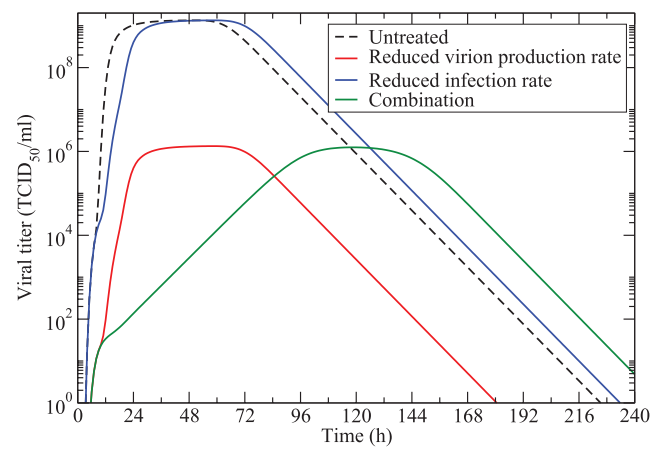
\includegraphics[width=\textwidth]{treatm1000.png}
    \end{subfigure}
    \begin{subfigure}{0.35\textwidth}
    
    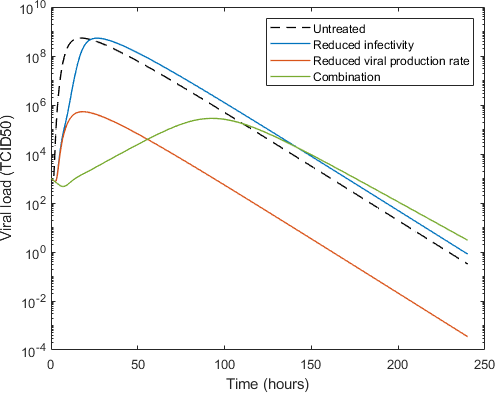
\includegraphics[width=\textwidth]{treat1000.png}
    \end{subfigure}
   
    
    \caption{\small The viral load curve under the original (left) and altered (right) models. The dose for each simulation is 10, 100, and 1000 $\mathrm{IC}_{50}$ in order from top to bottom}
    \label{fig:my_label}
\end{figure}

Figure 3 shows some of the heat maps for the peak viral load at different doses of pairs of drugs as predicted by the original and altered models. In our study using the altered model, we only explored doses up to $10^3 \hspace{1mm} \mathrm{IC}_{50}$ as opposed to $10^4 \hspace{1mm} \mathrm{IC}_{50}$ in the Melville et al. paper. This still allows us to capture the interesting behaviour of the model. The black line on the figures from the Melville et al. study is the line where we would theoretically expect the infection to be treated by the drug therapy.$^{[8]}$  Under both models the general trend for most pairs of drugs seems to be that the peak load is reduced as we move radially out from the origin. Exceptions to this are pairs where one of the drug acts to reduce $\beta$ under the altered model. This is in agreement with our observations from figure 2, however, in the original model it seems to be that at some point such a drug would in fact have the effect of reducing the peak viral load, as opposed to simply shifting this maximum to the right. The other notable exception are pairs where one drug acts to increase the eclipse phase duration under the original model. However, as the authors of that paper mention, this is due to a limitation where increasing $\tau_E$ can push the time of the peak viral load beyond the simulation time. In our study we improved on their method by scaling the simulation time with the drug doses which allowed us to avoid this problem. There are some dark spots visible on some of the maps taken from the Melville et al. study. They did not address these directly but we may assume that they are numerical artifacts. 

Figure 4 includes some of the heat maps for the infection duration as predicted by each model. Again, here we see what might be considered the 'standard' behaviour with the infection timescale decreasing radially until the infection is cured (infection duration is zero). Examples of this pattern are the $\beta_2-p$, and $\beta_2-c$ maps. We also see very similar behaviour predicted by the two variations for the $\beta_2-\tau_E$ treatment up until doses of $>  10 \hspace{1mm} \mathrm{IC}_{50}$ where the implementation of the original model presumably runs into the same computational issue as in the viral peak calculations. It is worth noting that at some doses the infection duration was found to be one or even two orders of magnitude higher that ten days (the highest point on the colourmap axis) with the altered model. This was not mentioned in the Melville et al. study, however it is reasonable to expect that this is also the case in the original model. In such cases the infection would also be very slow to surpass the $10^4 \hspace{1mm} \mathrm{TCID}_{50}$ infection threshold. An infection that grows so slowly is likely to be suppressed by the host's immune system.$^{[23]}$ We see also a dramatic difference in the behaviour of combinations that include a drug acting to reduce $\beta$. In the altered model such treatments fail to cure to infection at any dose up to $10^3 \hspace{1mm} \mathrm{IC}_{50}$, while in the original the infection is cured. 

\begin{figure}
    \centering
    \begin{subfigure}{0.4\textwidth}
    
    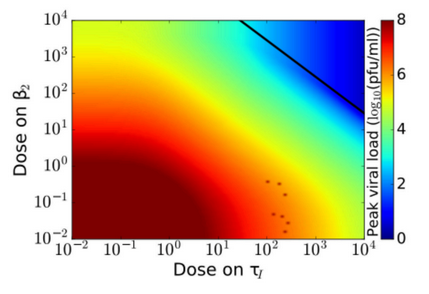
\includegraphics[width=\textwidth]{MBeta2TauIP.png}
    \end{subfigure}
    \begin{subfigure}{0.35\textwidth}
    
    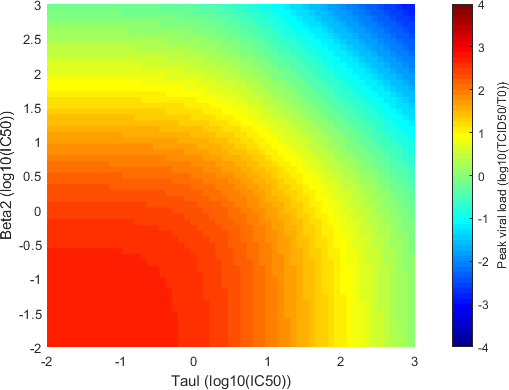
\includegraphics[width=\textwidth]{Beta2TauI_peaks.png}
    \end{subfigure}
    \begin{subfigure}{0.4\textwidth}
    
    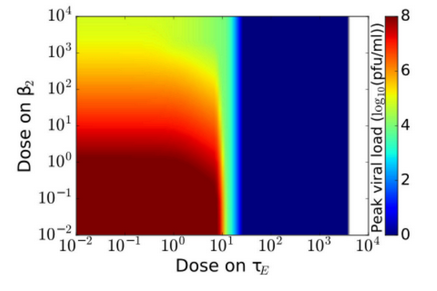
\includegraphics[width=\textwidth]{MBeta2TauEP.png}
    \end{subfigure}
    \begin{subfigure}{0.35\textwidth}
    
    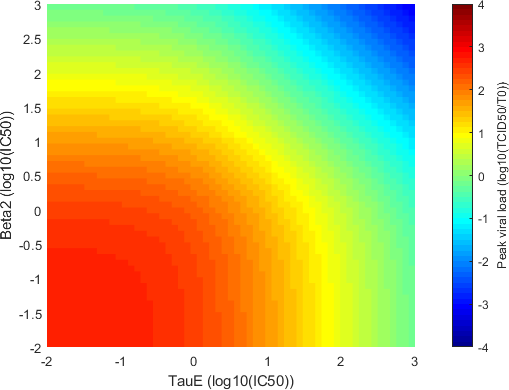
\includegraphics[width=\textwidth]{Beta2TauE_peaks.png}
    \end{subfigure}
    
    \begin{subfigure}{0.4\textwidth}
    
    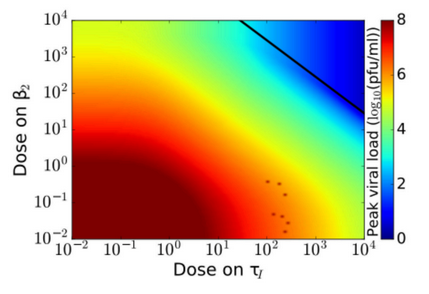
\includegraphics[width=\textwidth]{MBeta2TauIP.png}
    \end{subfigure}
    \begin{subfigure}{0.35\textwidth}
    
    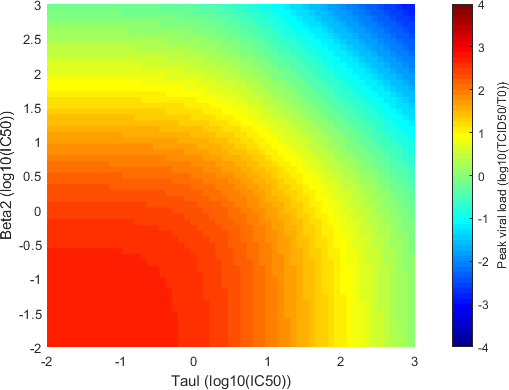
\includegraphics[width=\textwidth]{Beta2TauI_peaks.png}
    \end{subfigure}
    
      \begin{subfigure}{0.4\textwidth}
    
    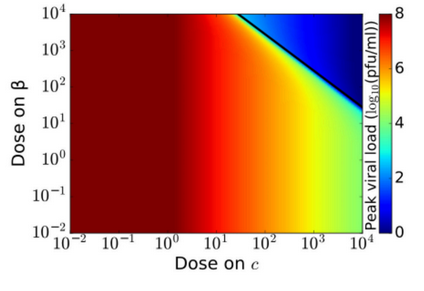
\includegraphics[width=\textwidth]{MBetaCP.png}
    \end{subfigure}
    \begin{subfigure}{0.35\textwidth}
    
    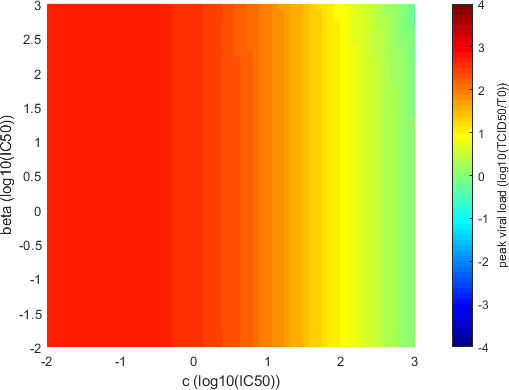
\includegraphics[width=\textwidth]{BetaC_peaks.png}
    \end{subfigure}
    \caption{\small The peak viral load under different models and drug combinations. Each pair has the results from the original model (left) and the altered model (right).}
    \label{fig:my_label}
    \end{figure}
  

\newpage

\begin{figure}[H]
    \centering
    \begin{subfigure}{0.4\textwidth}
    
    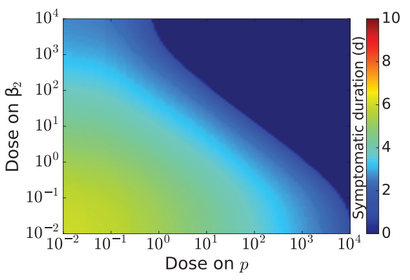
\includegraphics[width=\textwidth]{MBeta2PT.png}
    \end{subfigure}
    \begin{subfigure}{0.35\textwidth}
    
    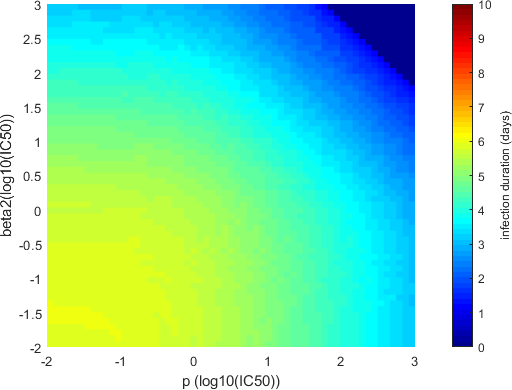
\includegraphics[width=\textwidth]{Beta2P_times.png}
    \end{subfigure}
    
    \begin{subfigure}{0.4\textwidth}
    
    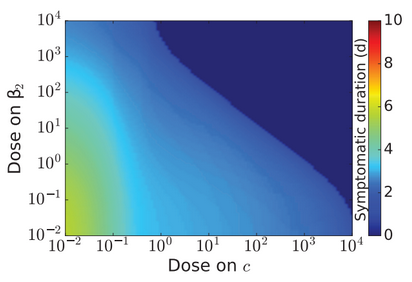
\includegraphics[width=\textwidth]{MBeta2CT.png}
    \end{subfigure}
    \begin{subfigure}{0.35\textwidth}
    
    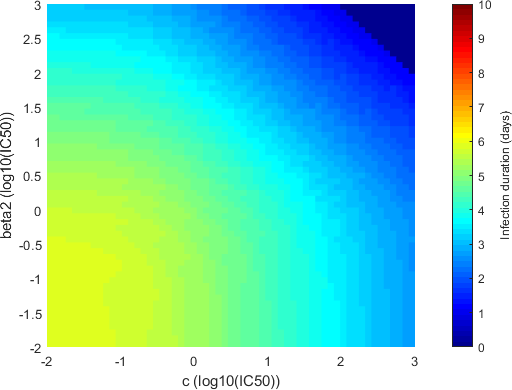
\includegraphics[width=\textwidth]{Beta2C_times.png}
    \end{subfigure}
    
    \begin{subfigure}{0.4\textwidth}
    
    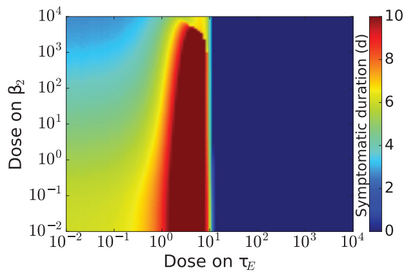
\includegraphics[width=\textwidth]{MBeta2TauET.png}
    \end{subfigure}
    \begin{subfigure}{0.35\textwidth}
    
    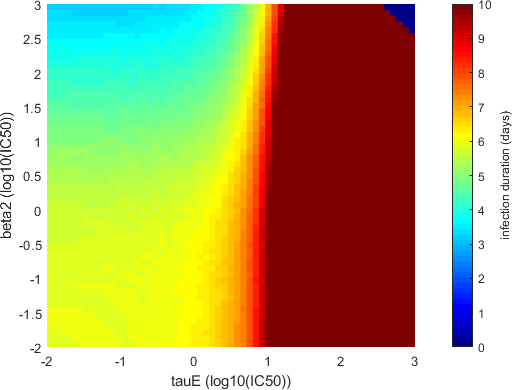
\includegraphics[width=\textwidth]{Beta2TauE_times.png}
    \end{subfigure}
    
     \begin{subfigure}{0.4\textwidth}
    
    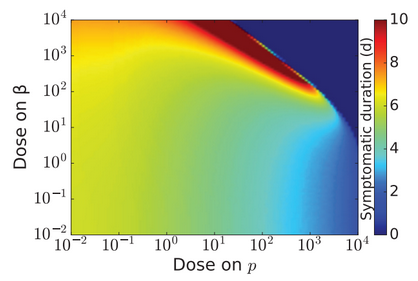
\includegraphics[width=\textwidth]{MBetaPT.png}
    \end{subfigure}
    \begin{subfigure}{0.35\textwidth}
    
    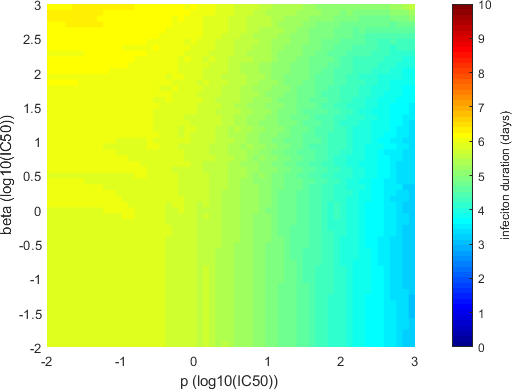
\includegraphics[width=\textwidth]{BetaP_times.png}
    \end{subfigure}
    
     \caption{\small The infection duration under different models and drug combinations. Each pair has the results from the original model (left) and the altered model (right).}
    \label{fig:my_label}
    
    \end{figure}
  

\newpage

\section*{Discussion}

Any conclusion about the robustness of the TIV model requires far more study. Here we have examined two variations which differ in only three parameters. There are, however, many other variations, some of which do away with a class of compartments entirely,$^{[9]}$ and some that add new compartments to account for immune response mechanisms from the host.$^{[12]}$ 

The small scope of this study notwithstanding, we find that the original and the altered models are in good qualitative agreement. One notable exception is the group of treatments which include a drug reducing the infectivity factor. In these cases the original model predicted that at higher doses, a drug acting to reduce $\beta$ would in fact have a significant effect on the peak viral load. This is despite what one might expect after observing the results from figure 2 where it appears that even at doses as high as $1000 \hspace{1mm} \mathrm{IC}_{50}$ such a drug has little to no impact on the peak viral load in either model, even in combination when another drug that reduces the viral production rate. 

This dissimilarity is present also in the predictions for infection duration in combination that contain a drug acting on $\beta$. Here both models show that doses of the drug acting on $\beta$ can have the effect of significantly increasing the infection timescale, however, in the original model, this is eventually cut off across a treatment line where the combination cures the infection. 

In non-linear systems such as these it can be difficult to speculate on the feedback systems at work, however one possible explanation for the behaviour of infectivity reducing drugs in the altered model is that the parameter $\beta$ may be simply determining the rate of the spread of the infection, without affecting the final viral load peak. It seems to be the case that both viral load and infected cell population peak in both the original and altered methods when target cells are depleted. This depletion is usually not gradual and slow, but occurs in one quick dip. So, if for example, reducing $\beta$ delays the time at which this dip occurs but does not significantly increase its timescale, then we might expect the results we have before us, since the terms $cV$ and $n_II_i/\tau_I$ are small before the dip. That is of course as long as $\beta$ is large enough such that we still have $R_0 > 1$. 



\section*{References}
\small{1. Panel on Antiretroviral Guidelines for Adults and Adolescents, 2018. Guidelines for the Use of Antiretroviral Agents in Adults and Adolescents Living with HIV. Department of Health and Human Services. Available at http://www.aidsinfo.nih.gov/ContentFiles/AdultandAdolescentGL.pdf. Accessed 19/02/2019 \newline
2. [Author], 1998. WHO Model Prescribing Information: Drugs Used in Leprosy, World Health Organization, Geneva. Available at http://apps.who.int/medicinedocs/pdf/h2988e/h2988e.pdf. Accessed 19/02/2019 \newline
3. Centre for Disease Control and Prevention, 2009. 2008-2009 Influenza Season Week 35 ending September 5, 2009, viewed 19/02/2019. https://www.cdc.gov/flu/weekly/weeklyarchives2008-2009/weekly35.htm\newline
4. Sanju\'an, R, abd Domingo-Calap, P. (2016). Mechanisms of viral mutation. Cell. Mol. Life Sci. 73. 4433-4448. doi:10.1007/s00018-016-2299-6 \newline
5. Villa, M., and L\"assig, M. (2017). Fitness cost of reassortment in human influenza. PLoS Pathog. 13:e1006685. doi: 10.1371/journal.ppat.1006685 \newline
6. Perelson, A. S., Rong, L., and Hayden, F. G. (2012). Combination antiviral therapy for influenza: predictions from modelling of human infections. J. Infect. Dis. 205,1642-1645. doi: 10.1093/infdis/jis265 \newline 
7. Dobrovolny, H. M., and Beachemin, C. A. (2017). Modelling the emergence of influenza drug resistance: the roles of surface proteins, the immune response and antiviral mechanisms. PLoS ONE 12:30180582 doi:10.1371/journal.pone.0180582 \newline 
8. Melville, K., Rodriguez, T., and Dobrovolony, H. M. (2018). Investigating DIfferent Mechanisms of Action in Combination Therapy for Influenza \newline
9. Hadjichrysanthou1, C., Cau\"et, E., Lawrence, E., Vegvari, C., de Wolf, F., Anderson, R. M., (2017). Understanding the within host dynamics of Influenza A virus: from theory to clinical implications. J. R. Soc. Interface 13:20160289, http://dx.doi.org/10.1098/rsif.2016.0289 \newline
10. Beauchemin, C. A. A, McSharry, J. J., Drusano, G. L., Nguyen, J. T., Went, G. T., Rebeiro, R. M., and Perelson, A. S. (2008). Modelling Amantadine Treatment of Influenza A Virus in  Vitro. J Theor Biol. 254(2): 439-451. doi:10.1016/j.jtbi.2008.05.031.\newline 
11. Cao, P., McCaw, J. (2017). The Mechanisms for Within-Host Influenza Virus Control Affect Model-Based Assessment and Prediction of Antiviral Treatment. Viruses. 9(8). doi: 10.3390/v9080197\newline
12.Nowak M., May R. M. 2000. Virus Dynamics: Mathematical Principles of Immunology and Virology \newline 
13. Centre for Disease Control and Prevention, 2018, Antiviral Drugs for Seasonal Influenza: Additional Links and Resources, viewed 20/02/2019, https://www.cdc.gov/flu/professionals/antivirals/links.htm \newline
14. Naesens, L., Stevaert, A., and Vanderlinden, E. (2016). Antiviral therapies on the horizon for influenza. Curr. Opin. Pharmacol. 20, 106-115. doi:10.1016/ j.coph.2016/08.003} \newline
15. Baccam, P., Beauchemin, C., Macken, C. A., Hayden, F.G., and Perelson, A. S. (2006). Kinetics of Influenza A virus infection in humans. J. Virol. 80,7590-7599. doi:10.1128/JVI.01623-05 \newline 
16. Handel, A. Jr., I. M. L., and Antia, R. (2007). Neurominidase inhibitor resistance in influenza: assessing the danger of its generation and spread. PLoS Comput. Biol. 3:e240. doi:10.1371/journal.pcbi.0030240 \newline 
17. Taylor, H. P., and Dimmock, N. J. (1985a). Mechanism of neutralization of influenza virus by secretory IgA is different from that of monomeric IgA or IgG. J. ExP. Med. 161, 198-209. doi:10.1084/jem/161.1.198 \newline
18. Taylor, H. P., and Dimmock, N. J. (1985b). Mechanisms of neutralization of influenza virus by IgM. J. Gen. Virol. 66(pt 4):903-907. doi:10.1099/0022-1317-66-4-903 \newline 
19. Fujimori, Y., Sato, T., Hayata, T., Nakayama, M., Nakayama, T., et al. (2012). Novel antiviral characteristics of nanosized copper(I) iodide particles showing inactivation activity against 2009 pandemic H1N1 influenza virus. Appl. Env. Microbiol. 78, 951-955. doi:10.1128/AEM.06284-11 \newline 
20. Heldt, F. S., Frensing, T., Pflugmacher, A., Gropler, R., Peschel, B., and Reichel, U. (2013). Multiscale Modelling of Influenza A virus infection supports the development of direct-acting antivirals. PLoS Comput. Biol. 9:e1003372. doi: 10.1371/journal.pcbi.1003372 \newline 
21. Zweerink, H., Skehel, S. C. J., Crumpton, M., and Askonas, B. (1997). Cytotoxic T cells kill influenza virus infected cells but do not distinguish between serologically distinct type A viruses. Nature 267, 354-356. doi: 10.1038/267354a0 \newline
22. Weiss, J. (1997). The Hill equation revisited: uses and misuses. Faseb j. 11, 835-841. doi: 10.1096/fasebj.11.11.9285481 \newline 
23. Beauchemin, C. A., and Handel, A. (2011). A review of mathematical models of influenza infections within a host or cell culture: lessons learned and challenges ahead. BMC Public Health 11(Suppl. 1):S7.doi: 10.1186/1471-2458-11-S1-S7 \newline 
24. Baron, S., Fons, M., Albrecht, T. (1996). Baron, Samuel, ed. Medical Microbiology (4th ed.). Galveston (TX): University of Texas Medical Branch at Galveston. ISBN 978-0963117212. PMID 21413306

\end{document}






\end{document}